\chapter{Cloud resourcebeheer, resource-allocatie en OpenStack}

In dit hoofdstuk wordt er dieper ingegaan op enkele belangrijke termen binnen cloud computing. Deze termen geven een beter idee over de werking van diverse cloud-systemen en de mogelijkheden die er zijn voor zowel de cloud-provider als de cloud-gebruiker, beiden besproken in Hoofdstuk~\ref{sec:what_is_cloud_computing} om hun cloud te beheren.

\section{Cloud resourcebeheer}
\label{sec:rmcloud}

Om ervoor te zorgen dat een cloud provider en een cloud-gebruiker steeds voldoen aan hun SLA, moeten beide partijen \textit{resource management} toepassen. Resource management heeft als doel de beschikbare bronnen zo efficiënt mogelijk te benutten, en precies voldoende bronnen te voorzien om \textit{underload} en/of \textit{overload} te vermijden.

\subsection{Resourcebeheer: de mogelijkheden}

Het doel van een cloud provider is het efficiënt beheren van de infrastructuur van het datacenter. Onderdelen hiervan zijn bijvoorbeeld \textit{balanced load} waarbij resources op een welbepaalde manier worden toegekend zodat het gebruik gebalanceerd is over alle resources van dat type, \textit{fault tolerance} waarbij de resources worden toegekend zodat de impact van het falen van een onderdeel minimaal blijft, of \textit{energy use minimization} waarbij de plaatsing van taken of jobs over resources zo gebeurt dat de energiekosten minimaal zijn. Een eventuele combinatie van bovenstaande onderdelen aan de hand van prioriteiten is mogelijk en de cloud provider kan ook bepaalde onderdelen koppelen aan verschillende operationele condities. Een voorbeeld van het laatste is het minimaliseren van het energieverbruik tijdens perioden met lage belasting, maar bij hogere belasting overschakelen naar balanced load in plaats van energy use minimization.

Een cloud-gebruiker heeft meestal een SLA met zijn eigen eindgebruikers met andere management doelen dan de cloud provider ten opzichte van zijn cloud-gebruikers. Hij maakt gebruik van de elasticiteit van cloud-omgevingen om zo extra resources te reserveren tijdens perioden met een hogere werklast en resources vrij te geven in perioden met minder werklast.

\subsection{Schalen}

Een cloud-gebruiker kan in twee probleemsituaties terecht komen indien hij verkeerd gebruikmaakt van de elasticiteit van cloud-omgevingen: \textit{over-provisioning} en \textit{under-provisioning}. Over-provisioning betekent dat de cloud-gebruiker meer resources ter beschikking heeft dan nodig met een hogere kost als gevolg. Doordat cloud computing ook een ``business'' is, zorgt dit voor nadelige effecten bij  zowel de cloud-gebruiker als eventuele eindgebruikers. Anderzijds betekent under-provisioning dat de cloud-gebruiker te weinig resources ter beschikking heeft, waardoor hij bijvoorbeeld performantiecriteria in de SLA met zijn eindgebruiker niet kan nakomen. Ook dit is een zeer nadelig effect voor beide partijen aangezien een eindgebruiker dan langer moet wachten op een antwoord (langere antwoordtijd) of geen antwoord krijgt door het falen van componenten.

Schalen van de beschikbare resources (of gebruik maken van de elasticiteit van een cloud-omgeving) voorkomt grotendeels de twee bovenstaande nadelige effecten. Hierin worden twee grote categorieën onderscheiden, statisch of periodiek en horizontaal of verticaal schalen. Bij statisch schalen worden er meer fysieke servers voorzien maar de tijd om deze te ordenen, te configureren en op te starten zal niet reactief genoeg zijn om een snelle stijging van de werklast te kunnen verwerken. Het gevolg hiervan is eerst een under-provisioning en nadien een over-provisioning omdat de opstart te lang duurt en het verlagen van het aantal resources pas na een bepaalde tijd van mindere activiteit zal worden uitgevoerd. Bijgevolg zorgt dit voor een slechtere performantie in het begin, door de under-provisioning, en een te hoge kostprijs achteraf door de over-provisioning.
Elastisch schalen daarentegen voorziet een stijging in resources met kleine stappen wat het systeem veel reactiever en kost-efficiënter maakt. Een belangrijke opmerking hierbij is dat het systeem zo ontworpen moet zijn dat het kan schalen, of met andere woorden, nuttig gebruik kan maken van de extra verkregen resources. Een SQL-databank is een voorbeeld van een minder schaalbare toepassing~\cite{Vaquero2011} omdat het gebruikmaakt van transacties die het gehele gebeuren blokkeren tot er een \textit{commit} wordt uitgevoerd. Het toekennen van extra resources heeft hier dus weinig nut omdat de toegang tot de gegevens geblokkeerd blijft.

In Figuur \ref{fig:scaling1} worden twee grafieken weergegeven die de toegekende resources weergeven bij statisch of elastisch schalen. Zoals te zien is, hangt statisch schalen sterk af van eventuele voorspellingen van de werklast waardoor het minder performant is bij pieken. Ook de nadelige effecten van under- en over-provisioning worden duidelijk weergegeven in de linkergrafiek. De rechtergrafiek weerspiegelt de kost-efficiëntie en performantie bij elastisch schalen en voor dit scenario is het duidelijk de aangewezen werkwijze om te schalen.


\begin{figure}
	\centering
	\captionsetup{justification=centering}
	\begin{subfigure}{\textwidth}
		\centering
		\centerline{
			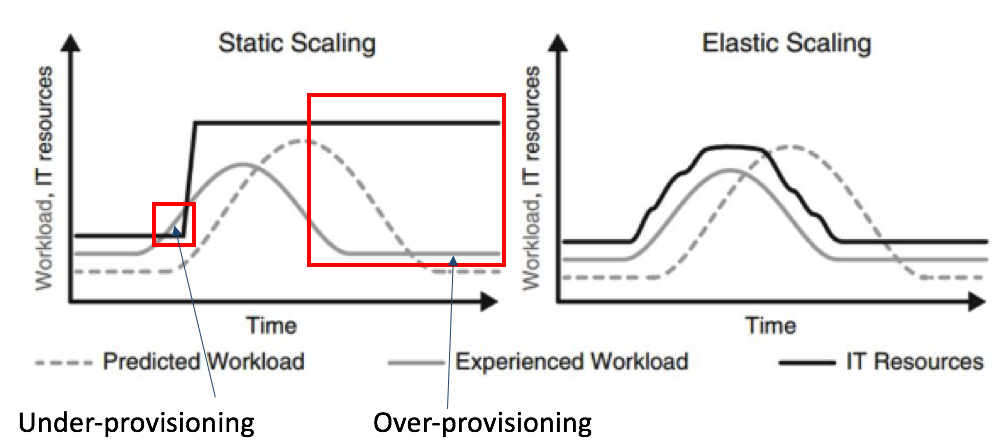
\includegraphics[scale=0.47]{scaling_1}
		}
	\end{subfigure}
	\caption{Statische vs. elastische schaling~\cite{Simoens}.}
	\label{fig:scaling1}
\end{figure}

Naast statisch of elastisch schalen kan er ook verticaal of horizontaal geschaald worden. Verticaal schalen wordt omschreven als het toevoegen van extra hardware zoals meer CPU-kracht, extra geheugen en opslag, etc. De voordelen zijn onder andere dat elke applicatie hier gebruik van kan maken omdat dit geen speciale architectuur vereist. Daarnaast omvat het een weinig risicovolle en minder complexe operatie dan horizontaal schalen en ten slotte is de kost ook redelijk in vergelijking met algoritmische verbeteringen. De nadelen wegen echter iets meer door dan de voordelen. Zo is er mogelijks een \textit{downtime} als er fysieke hardware wordt toegevoegd en is het niet zeker dat de applicatie gebruik kan maken van de nieuwe hardware. Een voorbeeld van dat laatste is een \textit{single-threaded} applicatie waarbij het toevoegen van extra CPU-kernen de applicatie niet zal versnellen en bijgevolg weinig nut heeft. Het is ook veel moeilijker om te \textit{downgraden} bij een dalende werklast en bovendien is er een absolute bovenlimiet doordat de onderliggende hardware van de fysieke node beperkt is.

Horizontaal schalen voegt extra fysieke- of applicatienodes toe in plaats van deze te upgraden waardoor een veel hogere capaciteit mogelijk is dan de grootste beschikbare enkelvoudige node. Een belangrijk voordeel is de hoge kost-efficiëntie omdat het elastisch schalen toelaat. De enige vereiste is dat de applicatie of toepassing die erop draait een gedistribueerde architectuur moet bevatten zodat verschillende nodes dezelfde functionaliteit van een applicatie kunnen uitvoeren. Meestal zijn zulke nodes volledig identiek geconfigureerd --zelfde hardware resources, zelfde besturingssysteem, zelfde software-- waardoor ze homogeen zijn. De homogeniteit van bepaalde nodes is een zeer belangrijke eigenschap bij horizontaal schalen omdat hierdoor \textit{round-robin load balancing} goed werkt en het maakt capaciteitsplanning en auto-schalen veel eenvoudiger dan bij heterogene nodes. Figuur \ref{fig:scaling2} geeft een overzicht van verticaal en horizontaal schalen.

\begin{figure}
	\centering
	\captionsetup{justification=centering}
	\begin{subfigure}{\textwidth}
		\centering
		\centerline{
			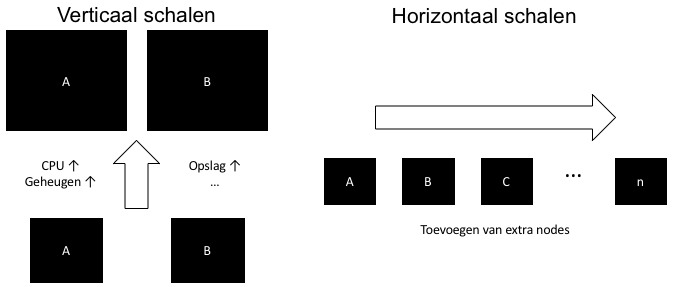
\includegraphics[scale=0.45]{horizontal_vertical_scaling}
		}
	\end{subfigure}
	\caption{Verticaal vs. horizontaal schalen van cloud resources}
	\label{fig:scaling2}
\end{figure}

\section{Resource-allocatie}
\label{sec:res_allocation}

\textit{Resource allocation} is een onderdeel van een overlappend concept samen met \textit{resource provisioning} en \textit{resource scheduling}~\cite{Yousafzai2016}. Resource provisioning en resource-allocatie zorgen voor het toekennen van resources van een cloud provider aan een cloud-gebruiker in een concurrerende omgeving van groepen programma's of gebruikers. Resource scheduling geeft een overzicht weer van welke resources er beschikbaar zijn en welke er gedeeld worden op bepaalde tijdstippen om zo zware rekentaken te plannen. Samengevat beschrijven deze drie termen het bepalen van wanneer rekenactiviteit moet gestart of gestopt worden, gebaseerd op voorgaande activiteiten en relaties alsook op de \textit{gealloceerde resources} en de duur van de activiteit.

In het algemeen bepaalt een cloud-gebruiker de hoeveelheid en het type van de resources die hij nodig heeft en zal de cloud provider deze aangevraagde resoures toewijzen in hun datacenters. Bij het bepalen van de hoeveelheid en het type van de resources moet er rekening gehouden worden met eventuele vereisten zoals bijvoorbeeld de maximale duur van een taak. Zoals te zien in Figuur \ref{fig:allocation1} beschrijft het cloud resource-allocatie mechanisme de beslissing in hoeveel, welke, waar en wanneer de beschikbare resources moeten toegekend worden aan de cloud-gebruikers. Dankzij de elasticiteit van cloud omgevingen kan een cloud-gebruiker resources dynamisch aanvragen en vrijgeven.

\begin{figure}
	\centering
	\captionsetup{justification=centering}
	\begin{subfigure}{\textwidth}
		\centering
		\centerline{
			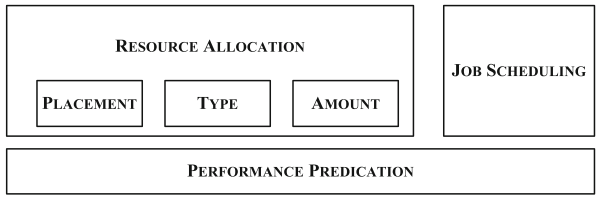
\includegraphics[scale=0.6]{allocation_overview}
		}
	\end{subfigure}
	\caption{Basisoverzicht van het resource-allocatie mechanisme.}
	\label{fig:allocation1}
\end{figure}

Cloud providers en cloud-gebruikers proberen uiteraard zoveel mogelijk winst te maken. Een cloud provider poogt dit door zoveel mogelijk virtuele machine's (VM's) uit te rollen op elke fysieke machine zodat de inkomsten hoog zijn en de investeringen laag. Een logisch gevolg hiervan is dat te veel VM's uitrollen op een fysieke machine kan leiden tot performantiedegradatie waardoor de cloud-gebruikers minder tevreden zijn. Cloud users daarentegen willen hun kost minimaal houden voor een maximale performantie, wat betekent dat ze efficiënt  de nodige resources zullen reserveren voor hun applicatie.

Doordat de datacenters van cloud providers heterogeen toenemen en dus bestaan uit verschillende generaties van hardware, zullen verschillende cloud-gebruikers heterogene resources van de cloud provider gebruiken (en delen met andere cloud-gebruikers) zonder veel inzicht in de infrastructuur met als nadelig gevolg dat het hele systeem onvoorspelbaar wordt. Het doel van resource-allocatie is zorgen voor efficiënte cloud-services, waarbij efficiënt staat voor het toekennen van de juiste resources aan de juiste applicatie op het juiste tijdstip. Hierdoor kunnen applicaties deze resources nuttig gebruiken.

\subsection{Indeling van cloud resource-allocatie schema's}

\begin{figure}
	\centering
	\captionsetup{justification=centering}
	\begin{subfigure}{\textwidth}
		\centering
		\centerline{
			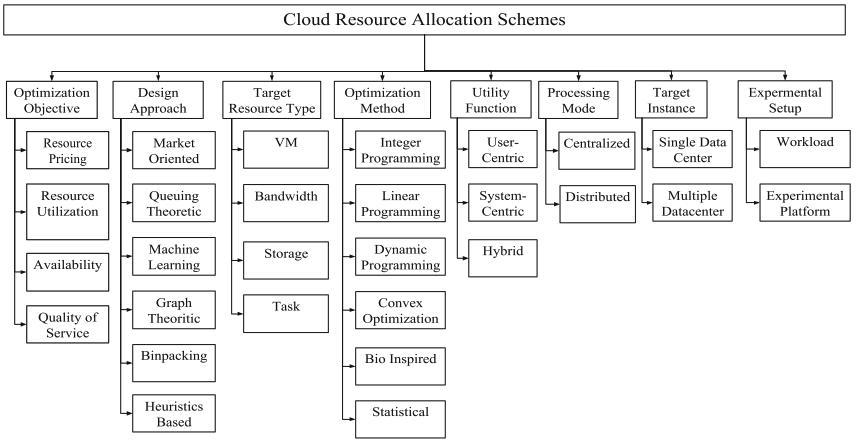
\includegraphics[scale=0.5]{taxonomyCRAS}
		}
	\end{subfigure}
	\caption{Indeling van resource-allocatie schema's voor cloud computing~\cite{Yousafzai2016}.}
	\label{fig:taxonomyCRAS}
\end{figure}

Zoals weergegeven in Figuur \ref{fig:taxonomyCRAS} kunnen de cloud resource-allocatie schema's onderverdeeld worden in acht categorieën~\cite{Yousafzai2016}. Deze worden hieronder per categorie kort besproken.

\subsubsection{Optimalisatiedoel (\textit{Optimization objective})}

De huidige resource-allocatie schema's pogen vier optimalisatiedoelen te volbrengen: \textit{Resource pricing} formuleert prijsmodellen om het algemeen verbruik van cloud resources te verbeteren waardoor cloud resources  gekocht, verkocht en geruild kunnen worden met andere cloud providers en/of cloud-gebruikers. \textit{Resource utilization} maximaliseert het gebruik van de virtuele en fysieke resources voor een betere performantie en is zeer gerelateerd met energieconsumptie. \textit{Availability} verzekert een bepaalde beschikbaarheid tijdens een contractuele periode door het dupliceren van taakuitvoering op resources of het dupliceren van data op verschillende geografische locaties, om zo om te kunnen gaan met x-voudige \textit{failures}. \textit{Quality of Service} zorgt voor een snelle response-tijd, weinig latency, etc.

\subsubsection{Ontwerpbenadering (\textit{Design approach})}

De ontwerpbenadering representeert het onderliggende model van de resource-allocatie en komt voor in vijf verschillende types. Het marktgeoriënteerd model (\textit{market-oriented}) benadert de functies van het vraag en aanbod systeem. Het \textit{queuing theoretic model} voorspelt verschillende performantiemetrieken en bijgevolg de nodige resources om de werklast te kunnen verwerken. \textit{Machine learning models} bekijken de resource-allocatie als een voorspellingsfunctie waarbij resultaten worden verwerkt met statistische technieken om zo verschillende patronen te ontdekken van bijvoorbeeld aanvragen, onzekerheidsfactoren, etc. \textit{Graph theoretic models} abstraheren cloud-systemen en zijn componenten voor het opstellen van modellen alsook voor het optimaliseren van de resource-allocatie aan de hand van grafen waarin de taken en de \textit{workflow} worden weergeven. Het \textit{bin packing model} plaatst verschillende items in een minimaal aantal \textit{bins} en dat wordt hier gebruikt om VM's te combineren op de fysieke nodes en om vrijgegeven resources consequent samen te nemen met als voordeel een efficiënter energieverbruik.
Samengevat bevindt het cloud resource-allocatie probleem zich in de NP, NPC en NP-hard complexe klassen. Oplossingen baseren zich daarom op heuristische methoden, die minder complex en sneller zijn, om dit probleem op te lossen.

\subsubsection{Type van doel-resource (\textit{Target resource type})}

Het \textit{target resource type} bepaalt hoe de extra resources worden afgeleverd aan de cloud-gebruiker of eindgebruiker. Afhankelijk van de vraag kan er bijvoorbeeld een extra VM ter beschikking worden gesteld, extra opslagruimte of bandbreedte voorzien worden, etc.

\subsubsection{Optimalisatiemethode (\textit{Optimization method})}

De optimalisatiemethode beschrijft de mathematische formulering voor het resource-allocatie probleem om zo een optimale of bijna-optimale oplossing te bepalen. Doordat de vraag en budgetten van gebruikers steeds variëren zijn polynomiale tijdsalgoritmen ongeschikt voor het oplossen van dit probleem en worden er daarom verschillende optimalisatiemethoden gebruikt om bijna-optimale oplossingen te creëeren zoals \textit{integer programming}, genetische algoritmen, etc.

\subsubsection{Nutsfunctie (\textit{Utility function})}

De nutsfunctie bepaalt of het resource-allocatie schema een \textit{system-centric}, \textit{user-centric} of \textit{hybrid} nut volgt. Deze drie types beschrijven hoe de cloud zal reageren indien het geen nieuwe resources meer kan alloceren. Bij system-centric staat de cloud provider zijn performantie centraal, bij user-centric staan de cloud-gebruikers centraal en het hybride-type bevindt zich tussen beiden.

\subsubsection{Verwerkingsmodus (\textit{Processing mode})}

Het doel van de nutsfunctie kan behaald worden door een optimalisatiemethode te gebruiken in een oftewel gecentraliseerde processing modus of een gedecentraliseerde modus. De gedecentraliseerde modus heeft als voordeel dat het geen \textit{single-point of failure} is maar het kan, in vergelijking met de gecentraliseerde modus, geen globale informatiestatus bevatten.

\subsubsection{Doel-instantie (\textit{Target instance})}

De doel-instantie bepaalt of het resource-allocatie schema moet werken in een \textit{single data center (SDC)} of een \textit{multiple data center (MDC)} cloud omgeving.

\subsubsection{Experimentele setup (\textit{Experimental setup})}

Elk nieuw resource-allocatie schema wordt eerst getest in een experimentele omgeving waarbij telkens het platform en de werklast bepaald moeten worden.

\section{OpenStack: een open-source softwareplatform voor cloud computing}
\label{sec:Openstack}

OpenStack~\cite{OpenStack2017} is open-source cloud computing software voor het beheren en onderhouden van clouds. Het OpenStack project is gestart in 2010 door Rackspace en NASA die verantwoordelijk zijn voor de eerste versie van de code. Ondertussen is OpenStack al uitgegroeid tot een ruime community met ondersteuning van meer dan 150 bedrijven~\cite{Wuhib2012}.

\begin{figure}
	\centering
	\captionsetup{justification=centering}
	\begin{subfigure}{\textwidth}
		\centering
		\centerline{
			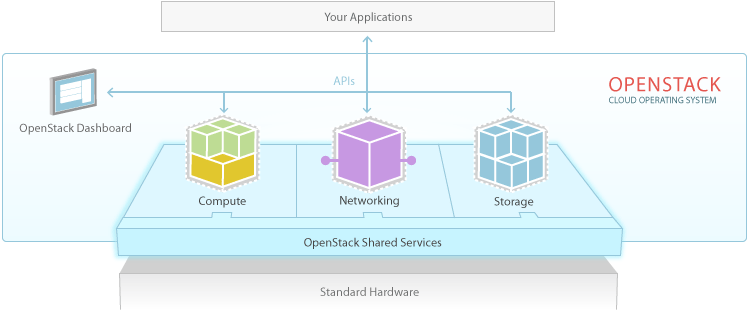
\includegraphics[scale=0.6]{openstack-software-diagram}
		}
	\end{subfigure}
	\caption{Architectuur van OpenStack~\cite{OpenStack2017}.}
	\label{fig:openstackdiagram}
\end{figure}

Figuur~\ref{fig:openstackdiagram} geeft de basisarchitectuur weer van OpenStack, waarbij duidelijk wordt dat het bestaat uit verschillende onafhankelijke componenten met een welgevormde \textit{Application Programming Interface} (API). OpenStack \textit{Compute} --Nova-- zorgt voor het beheren van VM's. \textit{Storage} zorgt dan weer voor het beheren van de opslag en \textit{Networking} zorgt voor de netwerkresources. Het OpenStack \textit{Dashboard} is een webinterface waarmee de 3 bovenstaande blokken van componenten beheerd worden, zoals het starten of stoppen van VM's, virtuele netwerktopologieën maken, etc.

Naast de vier aanwezige basiscomponenten in Figuur~\ref{fig:openstackdiagram}, bestaan er nog verschillende andere componenten die deel uitmaken van het OpenStack project. Zo zijn er de \textit{Orchestration}-services Heat~\cite{OpenStack2017g}, de Telemetry-Services~\cite{OpenStack2017h} \textit{Ceilometer} en \textit{Aodh}, etc. Bovendien bestaan er naast componenten ook andere toepassingen die ontwikkeld zijn voor en door OpenStack. Zo is er bijvoorbeeld het \textit{Heat Orchestration Template} (HOT) ~\cite{OpenStack2017f} formaat, ontwikkeld door community van OpenStack voor het aanmaken en configureren van verschillende onderdelen in Heat, Ceilometer, Nova, Neutron, etc.

Op dit ogenblik bevindt OpenStack zich in een vijftiende release, Ocata genaamd.\footnote{Februari 2017} Deze release is de opvolger van Newton en brengt enkele verbeteringen aan zoals betere stabiliteit en een versterkte \textit{core}-infrastructuur maar ook enkele nieuwe functies zoals de integratie van containers~\cite{Cathey2017}.